\documentclass{beamer}
\usetheme{Madrid}

\usepackage[yyyymmdd]{datetime}
\usepackage{fontspec}
\usepackage{fontenc}
\usepackage{amssymb}
\usepackage{ulem}
\usepackage{cite}
\usepackage{multirow}
\usepackage{mathtools}
\usepackage{amsmath}
\usepackage{float}
\usepackage{graphicx}
%\usepackage{url}
\usepackage{hyperref}
\usepackage{caption}
\usepackage{appendixnumberbeamer}
%\usepackage[svgnames]{xcolor}
%\usepackage{xstring} % to define myund
\usepackage[lithuanian]{babel}
%\usepackage{lineno}
\graphicspath{ {images/} }

\renewcommand{\dateseparator}{-}
\renewcommand{\abstractname}{Santrauka}
\renewcommand{\contentsname}{Turinys}
\renewcommand{\figurename}{Pav}
\renewcommand{\refname}{Literatūra}
\renewcommand{\tablename}{Lentelė}
\renewcommand{\listfigurename}{Paveikslėlių sąrašas}
\renewcommand{\listtablename}{Lentelių sąrašas}

\DeclareCaptionLabelFormat{numfirst}{#2~#1}

\newcommand{\textblue}[1]{{\color{Blue}#1}}
\newcommand{\textred}[1]{{\color{Red}#1}}
\newcommand{\comment}[1]{\newline\textblue{#1}\newline}
\newcommand{\commentNL}[1]{\textblue{#1}\newline}
\newcommand{\commentMA}[1]{\newline\textred{#1}\newline}
\newcommand{\pT}{\mathit{p}_{\mathrm{T}}}
\newcommand{\etaSC}{\eta_{\mathrm{SC}}}
\newcommand{\pTl}{\mathit{p}_{\mathrm{T\;Lead}}}
\newcommand{\pTsl}{\mathit{p}_{\mathrm{T\;Sublead}}}
\newcommand{\ET}{\mathit{E}_{\mathrm{T}}}
\newcommand{\refeqq}[1]{(\ref{#1})}
\newcommand{\Lumi}{{\cal L}_\mathrm{int}}
\newcommand{\pb}{$\mathrm{pb}$}
\newcommand{\fb}{$\mathrm{fb}$}
\newcommand{\GeV}{$\mathrm{GeV}$}
\newcommand{\TeV}{$\mathrm{TeV}$}
\newcommand{\invfb}{$\mathrm{fb}^{-1}$}
\newcommand{\invpb}{$\mathrm{pb}^{-1}$}
\newcommand{\ltq}[1]{{\quotedblbase{}#1\textquotedblleft{}}}
\newcommand{\WJets}{\mathit{W}+\mathrm{Jets}}
\newcommand{\emu}{\mathit{e}\mu}
\newcommand{\ee}{\mathit{ee}}
\newcommand{\mumu}{\mu\mu}
\newcommand{\WW}{\mathit{WW}}
\newcommand{\WWpm}{\mathit{W^{\,+}\!W^{\,-}}}
\newcommand{\ZZ}{\mathit{ZZ}}
\newcommand{\WZ}{\mathit{WZ}}
\newcommand{\gJets}{\gamma\! +\!\mathrm{Jets}}
\newcommand{\DYee}{\mathrm{DY} \! \rightarrow \! \mathit{ee}}
\newcommand{\DYtau}{\mathrm{DY} \! \rightarrow \! \tau\tau}
\newcommand{\dtW}{\mathit{tW}\! + \! \overline{\mathit{t}}\mathit{W}}
\newcommand{\QCD}{\mathit{QCD}}
\newcommand{\ttbar}{\mathit{t}\overline{\mathit{t}}}
\newcommand{\tbarW}{\overline{\mathit{t}}\mathit{W}}
\newcommand{\tW}{\mathit{tW}}



\title[Vasaros darbai]{Drell-Yan proceso tyrimui reikalingų duomenų apimties sumažinimas ir duomenų failų bibliotekos kūrimas}
\author[M.\ Ambrozas]{Marijus Ambrozas}
\date[2018-08-31]{2018 m.\ rugpjūčio 31 d.}

\begin{document}
\frame{\titlepage}


\begin{frame}
\frametitle{Turinys}

\begin{enumerate}
	\item Darbo planas
	\item Klasės \texttt{SelectedX} kūrimas
	\item Atrankos kodų kūrimas
	\item Įvykių atranka
	\item Susipažinimas su Tier3 centru
	\item Failų adresų bibliotekos kūrimas
	\item Rezultatai
	\item Artimiausi darbai
\end{enumerate}

\end{frame}


\begin{frame}[allowframebreaks]
\frametitle{Darbo planas}

\textbf{Tikslas:} Pagerinti programavimo įgūdžius, susipažinti su Seulo KISTI Tier3 centru.

\medskip
\textbf{Uždaviniai:}
\begin{enumerate}
	\item Sukurti klases SelectedX (X -- EE, MuMu, EMu), kuriose bus saugoma informacija apie įvykių atranką praėjusias daleles.
	\begin{itemize}
		\item Išsiaiškinti, kokius kintamuosius svarbiausia išsaugoti.
		\item Klases sukurti taip, kad eitų nesunkiai ir skaityti iš failo, ir į jį įrašinėti.
		\item Įsitikinti, ar viskas veikia.
	\end{itemize}
	\smallskip
	\item Parašyti kodus, kurie vykdo įvykių atranką, sukuria SelectedX klasės objektus ir įrašinėja juos į failą.
	\begin{itemize}
		\item Išsiaiškinti, kaip įvykių atranką vykdo kiti grupės mokslininkai ir jų kodais pasinaudoti kaip pradiniu tašku.
		\item Išbandyti kodus savo kompiuteryje su atsisiųstais nedideliais failais.
		\item Įsitikinti, ar į failus tikrai įrašoma informacija tik apie įvykių atranką praėjusias daleles.
		\item Paleisti skaičiavimus su Tier3 esančiais duomenų rinkiniais.
		\item Sukūrus failų biblioteką padaryti, kad kodai ją naudotų.
	\end{itemize}
	\item Susipažinti su Seulo KISTI Tier3 centru.
	\begin{itemize}
		\item Įsikelti GRID sertifikatą.
		\item Nusiklonuoti git saugyklą su kodais.
		\item Sužinoti, kur ir kaip saugomi duomenys, bei kur galiu duomenis saugoti pats.
		\item Sužinoti, kaip atsisiųsti duomenis.
		\item Išmokti naudotis TMUX.
	\end{itemize}
	\item Sukurti duomenų failų adresų biblioteką.
	\begin{itemize}
		\item Pažiūrėti, kaip su duomenų failų adresais tvarkosi kiti grupės mokslininkai.
		\item Gauti arba susidaryti visų reikalingų duomenų rinkinių sąrašą su adresais.
		\item Sukurti klasę, kuri saugotų visų reikalingų duomenų rinkinių adresus ir kitą svarbią susijusią informaciją, apjungiant anksčiau naudotą inputs.h kodą ir kitų mokslininkų kodus.
		\item Sudaryti galimybę duomenų rinkinių ieškoti pagal tekstinę įvestį (sukurti funkciją klasėje).
		\item Sudaryti galimybę įvykių atrankos kodus leistu su vienu ar keliais procesais paeiliui pagal tai, kokia tekstinė įvestis.
		\item Įsitikinti, ar viskas veikia (sukurti pasitikrinimo funkciją).
		\item Sukurti panašią klasę, tik skirtą tvarkytis su atsisiųstais atrinktų įvykių (SelectedX) failais.
	\end{itemize}
\end{enumerate}

\end{frame}


\begin{frame}
\frametitle{Klasės SelectedX kūrimas I}


Klasė išskirstyta į 3 subklases: \texttt{SelectedEE\_t}, \texttt{SelectedMuMu\_t} ir \texttt{SelectedEMu\_t}.
\begin{center}
	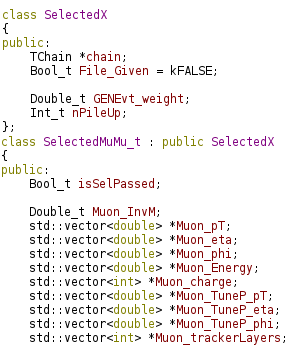
\includegraphics[width=0.47\textwidth]{SelectedX.png}
\end{center}

\end{frame}


\begin{frame}
\frametitle{Klasės SelectedX kūrimas II}
	
\begin{itemize}	
	\item Pežiūrėjau, kokių dydžių histogramas atlikęs įvykių atranką braižo KyeongPil Lee, bei kokie dydžiai naudojami korekcijoms (Rochester ir efektyvumo) ir juos sudėjau į reikiamas klases.
	\item Kad būtų galima klasės kintamuosius užpildyti naujomis vertėmis (kad galima būtų, pvz., įrašinėti į failą) sukūriau funkciją \texttt{CreateNew()}
	\item Kad būtų galima skaityti duomenis iš failo, sukūriau funkciją \texttt{CreateFromChain(TChain* chain)}, bei funkcijas \texttt{GetEvent(int i)}, \texttt{TurnOnBranches(TString brNames)}, \texttt{TurnOffBranches(TString brNames)}.
\end{itemize}

\end{frame}


\begin{frame}
\frametitle{Klasės SelectedX kūrimas III}

\begin{itemize}
	\item Sukūriau tris papildomas klases \texttt{LongSelectedX\_t}, kuriose galima išsaugoti visus su tam tikrų dalelių ($\ee$, $\mumu$ ar $\emu$) rinkiniu susijusius dydžius, kad galima būtų su šių klasių objektais vėliau padaryti pakartotinę įvykių atranką.
	\item Klases \texttt{SelectedX\_t} papildžiau funkcijomis \texttt{CreateFromLongSelectedX(LongSelectedX\_t *x, Bool\_t isSelPassed)}
\end{itemize}
\begin{minipage}{0.49\textwidth}
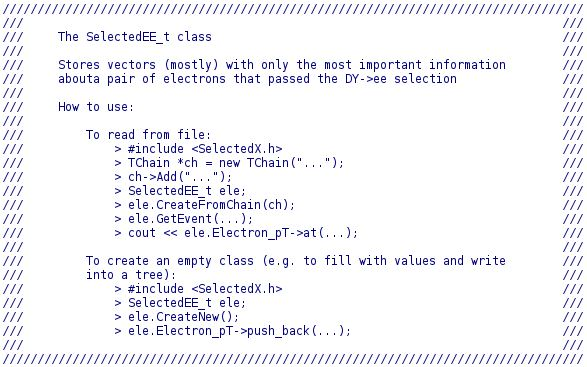
\includegraphics[width=\textwidth]{Selected.JPG}
\end{minipage}
\hfill
\begin{minipage}{0.49\textwidth}
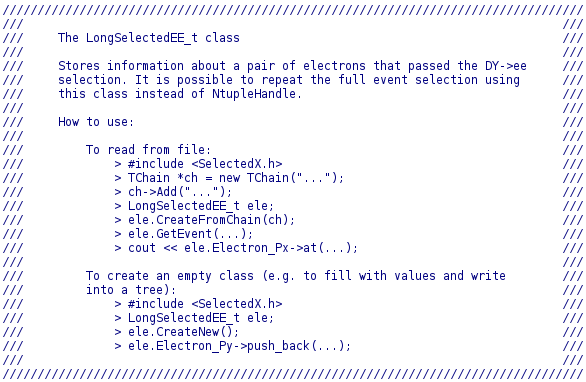
\includegraphics[width=\textwidth]{LongSelected.png}
\end{minipage}


\end{frame}

\begin{frame}[allowframebreaks]
\frametitle{Atrankos kodų kūrimas}

\begin{itemize}
	\item Kodų kūrimui kaip atspirties tašku naudojausi KyeongPil Lee ir Dalmin Pai įvykių atrankos kodais (\url{https://github.com/KyeongPil-Lee/DrellYan2016/tree/master/BkgEst/EventSelection})
	\item Pirmiausia parašiau kodus pavadinimu \texttt{MakeLongSelectedX.C,} kuriuose su atranką praėjusių dalelių informacija yra užpildomi \texttt{LongSelectedX\_t} klasių kintamieji. Šie kodai pritaikyti veikti tik su atsisiųstais nedideliais testiniais failais.
	\item Parašiau kitą kodą, kuris ima LongSelectedX duomenų (atrinktų įvykių) failą ir su juo vykdo pakartotinę įvykių atranką bei patikrina, ar tikrai visi šie įvykiai atranką praeina.
	\item Sukūriau kodą, kuris palygina atrinktų ir pakartotinai atrinktų duomenų failus.
	\item Parašiau kodus \texttt{MakeSelectedX.C}, kurie gali vykdyti įvykių atranką ne tik su testiniais failais, bei kurie pildo \texttt{SelectedX\_t} klasių kintamuosius (su tokiais atrinktais duomenimis pakartoti įvykių atrankos nebeišeina).
	\item \texttt{MakeSelectedX.C} išbandžiau su testiniais duomenų rinkiniais bei taip pat patikrinau, ar išsaugoti kintamieji sutampa su \texttt{MakeLongSelectedX.C} išsaugotais atitinkamais kintamaisiais.
	\item Atrinkdamas duomenis naudojausi KyeongPil Lee ir Dalmin Pai klasėmis (\url{https://github.com/KyeongPil-Lee/DrellYan2016/tree/master/BkgEst/EventSelection/header}): \texttt{NtupleHandle.h}, \texttt{Object.h} (šiek tiek modifikuota) ir \texttt{DYAnalyzer.h} (šiek tiek modifikuota).
	\item Įsitikinęs, kad viskas veikia su testiniais failais, pakeičiau \texttt{DYAnalyzer.h} buvusius failų adresus, kad atitiktų Tier3 centre esančių failų adresus ir paleidau skaičiuoti.
\end{itemize}

\end{frame}


\begin{frame}[allowframebreaks]
\frametitle{Įvykių atranka}

\begin{itemize}
	\item $\ee$ atranka:
	\begin{itemize}
		\item Trigeris \texttt{Ele23Ele12};
		\item \texttt{passMediumID};
		\item $\pTl>28$ \GeV, $\pTsl>17$ \GeV;
		\item $|\etaSC|<2.4$ ir $1.4442<|\etaSC|<1.566$;
		\item 2 išvardintus kriterijus atitinkantys elektronai, kurių $\mathit{m}_{\mathrm{inv}}>10$ \GeV.
	\end{itemize}
	\item $\mu\mu$ atranka:
	\begin{itemize}
		\item Trigeris \texttt{IsoMu24} arba \texttt{IsoTkMu24};
		\item \texttt{isHighPtMuon};
		\item \texttt{TrkIso<0.1}; 
		\item $\pTl>28$ \GeV, $\pTsl>17$ \GeV;
		\item $|\etaSC|<2.4$ ir $1.4442<|\etaSC|<1.566$;
		\item 2 priešingų krūvių išvardintus kriterijus atitinkantys miuonai, kurių $\mathit{m}_{\mathrm{inv}}>10$ \GeV;
		\item \texttt{vtxTrkChi2/Ndof<20};
		\item Kampas tarp miuonų \texttt{Inner} keturmačio impulso vektorių $\alpha<\pi-0.005$.
	\end{itemize}
	\item $\emu$ atranka:
	\begin{itemize}
		\item Trigeris \texttt{IsoMu24} arba \texttt{IsoTkMu24};
		\item Miuono \texttt{TrkIso<0.1}; 
		\item Abiejų dalelių $\pT>17$ \GeV, bet bent vienos iš jų $\pT>28$ \GeV;
		\item Abiejų dalelių $|\eta|<2.4$; $|\etaSC^{\mathit{e}}|<2.4$ ir $1.4442<|\etaSC^{\mathit{e}}|<1.566$;
		\item Elektronas, tenkinantis \texttt{passMediumID} reikalavimus;
		\item Po vieną išvardintus kriterijus atitinkančią dalelę, kurių $\mathit{m}_{\mathrm{inv}}>10$ \GeV;
		\item Atrinktasis miuonas būtinai turi būti tas, kuris sužadino trigerį.
	\end{itemize}
\end{itemize}

\end{frame}


\begin{frame}
\frametitle{Susipažinimas su Tier3 centru}

\begin{itemize}
	\item Įsikėliau GRID sertifikatą (du kartus, nes turėjau seną, kuris rugpjūčio mėn. nustojo galioti).
	\item Nusiklonavau git saugyklą (\url{https://github.com/marijusambrozas/DrellYan2016})
	\item Duomenys saugomi centre \texttt{/xrootd/store/user/dpai/\_v2p3\_/}. Duomenis iš išorės galima pasiekti prisijungus prie xrootd serverio (įvedus \texttt{xrd cms-xrdr.sdfarm.kr}, arba galima iškart kopijuoti pasinaudojus komanda \texttt{xrdcp}).
	\item Savo duomenims saugoti turiu vietą \texttt{/xrootd/store/user/mambroza/}
	\item Pramokau TMUX pagrindų. Tai yra ganėtinai patogu, nes galima turėti kelis terminalus vienu metu ir nutrūkus ryšiui TMUX sesija neišsijungia (paleidus skaičiuoti kodą, skaičiavimas nenutrūksta).
\end{itemize}

\end{frame}


\begin{frame}[allowframebreaks]
\frametitle{Failų adresų bibliotekos kūrimas}

KyeongPil Lee ir Dalmin Pai koduose duomenų failų rinkinys pasirenkamas kaip argumentą nurodant tam tikrą skaičių -- nepatogu, nes reikia vis iš naujo prisiminti, kokį procesą koks skaičius reiškia.

\begin{center}
	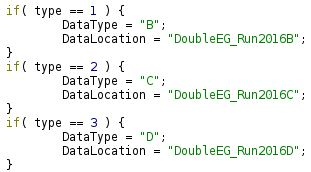
\includegraphics[width=0.6\textwidth]{oldAddress.JPG}
\end{center}
	
\end{frame}


\begin{frame}
\frametitle{Failų adresų bibliotekos kūrimas II}

Sukūriau klasę \texttt{FileMgr.h}. Procesus sunumeravau pasinaudodamas \texttt{typedef enum} panašiai, kaip buvo anksčiau naudotame kode \texttt{inputs.cc}.

\begin{center}
	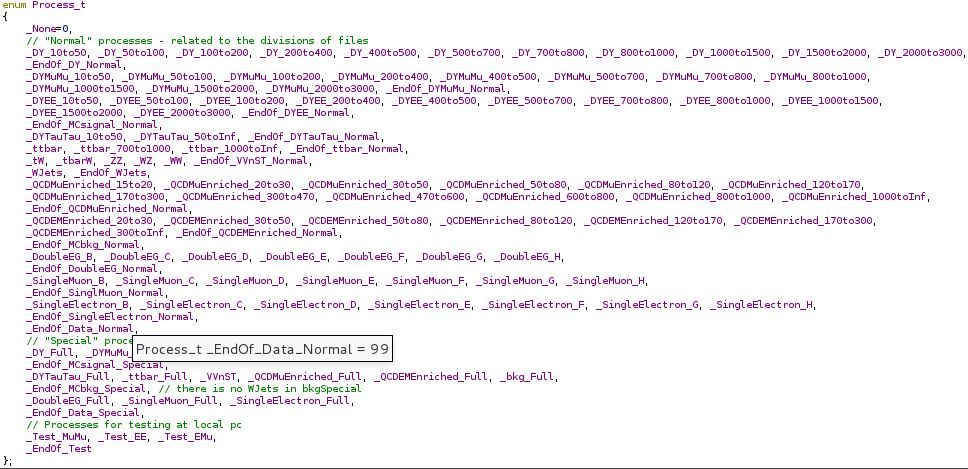
\includegraphics[width=0.95\textwidth]{enum.JPG}
\end{center}

\end{frame}


\begin{frame}
\frametitle{Failų adresų bibliotekos kūrimas III}

\begin{itemize}
	\item Gavau visų duomenų rinkinių sąrašą su jų adresais (juos jau panaudojau iš pradžių pakeisdamas failų adresus klasėje \texttt{DYAnalyzer.h}).
	\item Klasės kintamieji: \texttt{CurrentProc}, \texttt{Procname}, \texttt{Tag} (kad būtų suderinama su KyeongPil Lee duomenų rinkinių atskyrimu), \texttt{BaseLocation}, \texttt{FileLocation}, \texttt{FullLocation}, \texttt{TreeName}, \texttt{Type}, \texttt{Xsec}, \texttt{Wsum}, \texttt{nEvents}, \texttt{isMC}. 
	\item Sukūriau funkciją \texttt{GetProc(Process\_t pr, ..)}, kuri klasės kintamuosius užpildo argumente pateikto proceso informacija. Funkcija \texttt{ClearProc()} šią informaciją išvalo, o \texttt{NextProc} ją pakeičia sekančio proceso informacija.  
	\item Sukūriau funkciją \texttt{FindProc(TString search, ..)}, kuri pagal tekstinę įvestį grąžina ją atitinkančius procesus.
\end{itemize}

\end{frame}


\begin{frame}
\frametitle{Duomenų failų adresų bibliotekos kūrimas IV}

\begin{center}
	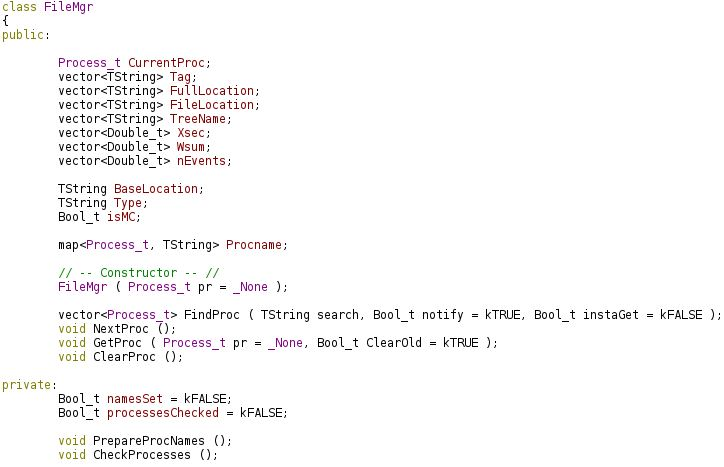
\includegraphics[width=0.99\textwidth]{filemgr.JPG}
\end{center}

\end{frame}


\begin{frame}
\frametitle{Duomenų failų adresų bibliotekos kūrimas V}

\begin{itemize}
	\item ROOT aplinkoje bei per funkciją \texttt{CheckProcesses()} patikrinęs, ar viskas veikia, pakoregavau kodus \texttt{MakeSelectedX.C}, kad naudotųsi šia klase.
	\item Sukūriau dar vieną labai panašią klasę \texttt{LocalFileMgr.h}, kuri skirta tvarkytis su atrinktų duomenų failais.
\end{itemize}

\begin{center}
	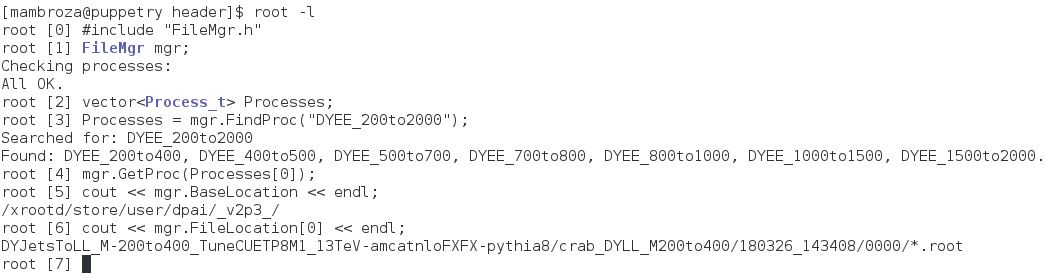
\includegraphics[width=1.02\textwidth]{MgrAtWork.JPG}
\end{center}

\end{frame}


\begin{frame}
\frametitle{Rezultatai}

\begin{itemize}
	\item Įvykių atrankos kodai su sukurta failų biblioteka veikia gerai.
	\item Po įvykių atrankos atsisiuntus atrinktų duomenų rinkinius:
	\begin{itemize}
		\item Atrinktų $\ee$ duomenų failai bendrai užima apie $3.5\; \mathrm{GB}$;
		\item Atrinktų $\mu\mu$  duomenų failai bendrai užima apie $4.8\; \mathrm{GB}$;
		\item Atrinkti $\emu$ duomenų failai bendrai užima apie $219\; \mathrm{MB}$;
	\end{itemize}
	\item Aptiktos problemos su šiais duomenų failais:
	\begin{itemize}
		\item \texttt{../crab\_DoubleEG\_RunHver2/../0000/ntuple\_skim\_452.root}
		\item \texttt{../crab\_SingleMuon\_RunG/../ntuple\_skim\_697.root}
		\item \texttt{../crab\_QCDMuEnriched\_Pt20to30/../ntuple\_skim\_117.root}
		\item \texttt{../crab\_QCDEMEnriched\_Pt120to170/../ntuple\_skim\_116.root}
	\end{itemize}
	\item Visų duomenų rinkinių įvykių skaičiai ir svorių sumos yra suskaičiuotos ir saugomos klasėje \texttt{FileMgr.h}
	\item Visi parašyti kodai saugomi \url{https://github.com/marijusambrozas/DrellYan2016/tree/master/SelectedX}
\end{itemize}

\end{frame}


\begin{frame}
\frametitle{Artimiausi darbai}

\begin{itemize}
	\item Pasidariau kodus, kurie iš atrinktų $\ee$ ir $\mu\mu$ įvykių sukuria histogramas ir jas įrašo į failus.
	\item Reikia pasirašyti kodus, kurie tas histogramas galėtų susumuoti ir išbrėžti, kad būtų galima daryti Drell-Yan proceso triukšmų įvertinimą MC ir $\emu$ metodais.
\end{itemize}

\end{frame}


\end{document}
